%%
%% Copyright 2007, 2008, 2009 Elsevier Ltd
%%
%% This file is part of the 'Elsarticle Bundle'.
%% ---------------------------------------------
%%
%% It may be distributed under the conditions of the LaTeX Project Public
%% License, either version 1.2 of this license or (at your option) any
%% later version.  The latest version of this license is in
%%    http://www.latex-project.org/lppl.txt
%% and version 1.2 or later is part of all distributions of LaTeX
%% version 1999/12/01 or later.
%%
%% The list of all files belonging to the 'Elsarticle Bundle' is
%% given in the file `manifest.txt'.
%%

%% Template article for Elsevier's document class `elsarticle'
%% with numbered style bibliographic references
%% SP 2008/03/01
%%
%%
%%
%% $Id: elsarticle-template-num.tex 4 2009-10-24 08:22:58Z rishi $
%%
%%
\documentclass[preprint,12pt,3p]{elsarticle}

%% Use the option review to obtain double line spacing
%% \documentclass[preprint,review,12pt]{elsarticle}

%% Use the options 1p,twocolumn; 3p; 3p,twocolumn; 5p; or 5p,twocolumn
%% for a journal layout:
%% \documentclass[final,1p,times]{elsarticle}
%% \documentclass[final,1p,times,twocolumn]{elsarticle}
%% \documentclass[final,3p,times]{elsarticle}
%% \documentclass[final,3p,times,twocolumn]{elsarticle}
%% \documentclass[final,5p,times]{elsarticle}
%% \documentclass[final,5p,times,twocolumn]{elsarticle}

%% if you use PostScript figures in your article
%% use the graphics package for simple commands
%% \usepackage{graphics}
%% or use the graphicx package for more complicated commands
%% \usepackage{graphicx}
%% or use the epsfig package if you prefer to use the old commands
%% \usepackage{epsfig}
\usepackage{amsmath}
%% The amssymb package provides various useful mathematical symbols
\usepackage{amssymb}
%% The amsthm package provides extended theorem environments
\usepackage{amsthm}
%% Code listings
\usepackage{listings}
\usepackage{algorithm}
\usepackage{algorithmic}

%% The lineno packages adds line numbers. Start line numbering with
%% \begin{linenumbers}, end it with \end{linenumbers}. Or switch it on
%% for the whole article with \linenumbers after \end{frontmatter}.
%% \usepackage{lineno}

%% natbib.sty is loaded by default. However, natbib options can be
%% provided with \biboptions{...} command. Following options are
%% valid:

%%   round  -  round parentheses are used (default)
%%   square -  square brackets are used   [option]
%%   curly  -  curly braces are used      {option}
%%   angle  -  angle brackets are used    <option>
%%   semicolon  -  multiple citations separated by semi-colon
%%   colon  - same as semicolon, an earlier confusion
%%   comma  -  separated by comma
%%   numbers-  selects numerical citations
%%   super  -  numerical citations as superscripts
%%   sort   -  sorts multiple citations according to order in ref. list
%%   sort&compress   -  like sort, but also compresses numerical citations
%%   compress - compresses without sorting
%%
%% \biboptions{comma,round}

% \biboptions{}

\begin{document}

\begin{frontmatter}

\title{Project Report: Inverse Problems}


\author{Kevin Marchais}
\ead{kevin.marchais@enseirb-matmeca.fr}

\author{Marcel Windpassinger}
\ead{smarcelw@gmail.com}

\author{Babacar Foune}
\ead{babsfoune@gmail.com}

\begin{abstract}
We are interested in finding the position of a heat source in the unit disc when given the resulting heat flux at the boundary. This question poses an inverse problem to calculating the heat distribution for given source coordinates. 

In the following report, we present a gradient method approach to approximate the heat source position using a finite element framework provided by FreeFem++ \cite{MR3043640}. We begin by outlining the problem details in section 1 and proceed with a breakdown of the gradient method in section 2. Section 3 deals with implementation specifics and section 4 showcases numerical results.
\end{abstract}

\end{frontmatter}

%%
%% Start line numbering here if you want
%%
% \linenumbers

%% main text
\section{Setting}
To begin, we specify the problem. Let $\Omega = B_0(1)$ be the unit disc in $\mathbb R^2$. A heat distribution with source $G\in C^1(\Omega)\cap C^0(\overline{\Omega})$ is a function $\phi\in H^1_0(\Omega)$ satisfying
\begin{equation}\label{eq:1}
	\Delta \phi = G 
	\hspace{30pt}\text{in }\Omega.
\end{equation}
Note that other choices for boundary values are also possible in principle, however they might necessitate changes for resulting formulations in the later chapters.

We presuppose that any heat source must have the form
\begin{equation}\label{eq:2}
	G(x_0,y_0) = \exp\left((x-x_0)^2+(y-y_0)^2\right),\text{ for all }x,y\in\overline{\Omega}
\end{equation}
i.e. that heat is radiating from a single point $(x_0,y_0)\in\Omega$. We suppose further that this point is unknown to the observer who can only measure the heat flux $\frac{\partial \phi}{\partial n}$ of the resulting distribution $\phi$ at the boundary $\partial\Omega$.

His task thus is: given a (potentially approximate) heat flux $g\in C^0(\partial\Omega)$, find the optimal solution $\left(\phi^*,(x^*,y^*)\right)\in \mathcal C\times\Omega$ to the minimization problem
\begin{align}\label{eq:3}
	 \underset{\mathcal C\times\Omega}{\min}\;I(\phi,(x_0,y_0))
	&=\frac{1}{2} 
		\int_{\partial\Omega}
			\left( \frac{\partial \phi^*}{\partial n} - g\right)^2 \mathrm{d}s\\
	\text{with }\Delta \phi^* 
	&= G(x^*,y^*)\label{eq:4}
\end{align}
for the heat distribution space $\mathcal C = \{ \phi\in H^1_0(\Omega)\:|\:\Delta \phi = G\text{ in }\Omega,\:\text{ with $G$ of the form (\ref{eq:2})}\}$.
\section{Gradient method approach}
In order to find a practical solution of the minimization problem (\ref{eq:3}-\ref{eq:4}) we have to subdivide the procedure into the following steps: in \textit{section 2.1} we use a variational approach to deduce a necessary condition for the minimizing heat distribution. In \textit{section 2.2} we take an adjoint equation approach in order to obtain necessary and sufficient conditions for a the heat coordinates. A combination of these two results in \textit{section 2.3} allows us to derive a gradient method in \textit{section 2.4}.

\subsection{Variational calculus ansatz}
Let $\widetilde{\phi}\in\mathcal{C}$ be an arbitrary perturbation of a distribution $\phi$ by a small parameter $\epsilon>0$. We define the gradient approximate $J_\epsilon$ of $I$ toward $\widetilde{\phi}$ by
\begin{equation}\label{eq:5}
	J_\epsilon(\phi) =
	\frac{1}{\epsilon}
	\left[
		I(\phi+\epsilon\widetilde{\phi})-I(\phi)
	\right].
\end{equation}
Using elementary operations, one can show that it holds
\begin{equation}\label{eq:6}
	J_\epsilon(\phi) =
	\frac{\epsilon}{2}\int_{\partial\Omega} \left(\frac{\partial\widetilde{\phi}}{\partial n}\right)^2 \mathrm{d}s
	\,+\,\int_{\partial\Omega} \frac{\partial\widetilde{\phi}}{\partial n} 
		\left(g-\frac{\partial\phi}{\partial n}\right) \mathrm{d}s.
\end{equation}
Thus, taking the limit $\epsilon\to 0$, we gain a necessary condition for the minimizer $\phi^*$:
\begin{equation}\label{eq:7}
	J_0(\phi^*) = 
	\int_{\partial\Omega} \frac{\partial\widetilde{\phi}}{\partial n} 
		\left(g-\frac{\partial\phi^*}{\partial n}\right) \mathrm{d}s
	= 0.
\end{equation}
Since $\widetilde{\phi}$ is arbitrary, we have shown that all directional derivatives of $I$ at $\phi^*$ must be zero. We can now conclude from the following two claims that this is already sufficient. 
\begin{itemize}
	\item \underline{first claim:} $\mathcal C$ is convex.\\
	Let $\alpha\in(0,1)$, $\phi_1,\phi_2\in\mathcal C$. Then
	\begin{equation*}
		\Delta \left(\alpha\phi_1 + (1-\alpha)\phi_2\right)
		= \alpha \Delta \phi_1 + (1-\alpha)\Delta\phi_2
		= (\alpha + 1 - \alpha)G = G.
	\end{equation*}
	\item \underline{second claim:} $I$ is convex.\\
	Indeed, $I$ is the composition $I = L\circ Q\circ D$, where\\
	$\:L=\int_{\partial\Omega}\cdot\,\mathrm ds$ is linear, $\:Q=\frac{1}{2}(\:\cdot\:)^2$ is quadratic, thus convex and $\:D=(\frac{\partial\,\cdot}{\partial n}-g)$ is linear.
\end{itemize}
As we find ourselves in the Hilbert space setting of $L^2$, we can make use of the scalar product $\left(\cdot,\cdot\right) = \left(\cdot,\cdot\right)_{L^2(\partial \Omega)}$ and note the necessary condition (\ref{eq:7}) as follows:
\begin{equation}\label{eq:8}
	\left(\nabla Q(D(\phi)),\frac{\partial \widetilde{\phi}}{\partial n}\right)
	\overset{!}{=}0,
\end{equation}
i.e. at the minimum $\phi^*$ the gradient of $Q\circ D$ has to be orthogonal to the outer heat flux of any perturbation $\widetilde{\phi}$.

\subsection{Lagrange Multiplier in $\mathcal C$}
In order to incorporate the auxiliary condition (\ref{eq:4}) into the minimization routine, we introduce the Lagrange multiplier $\lambda\in H^1(\Omega)$. We will see later why $H^1$ is a good choice.

Consider the first order linearization of (\ref{eq:4}):
\begin{equation}\label{eq:9}
	\Delta\left(\phi+\epsilon\widetilde{\phi}\right)
	= G(x_0,y_0)+\epsilon
		\left(\frac{\partial G}{\partial x_0}x_0+\frac{\partial G}{\partial y_0}y_0\right)
		+ \mathcal O(\epsilon^2).
\end{equation}
This directly yields
\begin{equation}\label{eq:10}
	\Delta\widetilde{\phi} 
	= \frac{\partial G}{\partial x_0}x_0+\frac{\partial G}{\partial y_0}y_0
\end{equation}
for any perturbation $\widetilde{\phi}$.
Testing (\ref{eq:10}) with $\lambda$ and integrating leads to
\begin{equation}\label{eq:11}
	\int_\Omega \lambda \left( 
		\Delta\widetilde{\phi} 
		- \frac{\partial G}{\partial x_0}x_0-\frac{\partial G}{\partial y_0}y_0
	\right)\,\mathrm{d}x
	= 0.
\end{equation}
We now integrate $\lambda\Delta \widetilde{\phi}$ by parts twice and obtain, noticing that $\widetilde{\phi}\in H^1_0$ is zero on the boundary, 
\begin{align}\label{eq:12}
	&\int_\Omega \widetilde{\phi} \Delta\lambda \:\mathrm{d}x
	-\int_\Omega\lambda \left( 
	 \frac{\partial G}{\partial x_0}x_0+\frac{\partial G}{\partial y_0}y_0
	\right)\,\mathrm{d}x\\
	+&\int_{\partial \Omega} \lambda \,\frac{\partial\widetilde{\phi}}{\partial n}\:\mathrm{d}s
	= 0,\nonumber
\end{align}
which must be fulfilled for all $\lambda$ and all $\widetilde{\phi}$, thereby giving us necessary and sufficient conditions on $(x_0,y_0)$. $\mathcal{C}$ is spanned by the linear, self-adjoint operator $\Delta$. We have only used the adjoint in the first part, therefore we call (\ref{eq:12}) pseudo adjoint equation.

\subsection{Application of the Lagrange multiplier to the necessary condition (\ref{eq:8})}
In order to find the minimum in $\mathcal{C}$, we need to combine conditions for the optimum and Lagrange multiplier. 
Subtracting pseudo adjoint equation and necessary condition on $\phi$ from each other, we obtain
\begin{align}\label{eq:13}
	&\int_\Omega \widetilde{\phi} \Delta\lambda \:\mathrm{d}x
	-\int_\Omega\lambda \left( 
	\frac{\partial G}{\partial x_0}x_0+\frac{\partial G}{\partial y_0}y_0
	\right)\,\mathrm{d}x\\
	+&\int_{\partial \Omega} \lambda \,\frac{\partial\widetilde{\phi}}{\partial n}\:\mathrm{d}s
	-\int_{\partial\Omega} \frac{\partial\widetilde{\phi}}{\partial n} 
		\left(g-\frac{\partial\phi^*}{\partial n}\right) \mathrm{d}s
	= 0,\nonumber
\end{align}
from which we can find this particular choice for $\lambda$:
\begin{itemize}
	\item[1)] $\Delta\lambda=0$ in $\Omega$,
	\item[2)] $\lambda=g-\frac{\partial\phi}{\partial n}$ on $\partial\Omega$,
	\item[3)] $\int_{\Omega}\lambda\frac{\partial G}{\partial x_0}
			  =\int_{\Omega}\lambda\frac{\partial G}{\partial y_0} = 0,$
\end{itemize}
causing all individual integrals to vanish or to eliminate each other respectively.
Together with 
\begin{itemize}
	\item[4)] $\Delta\phi=G$,
\end{itemize}
we have thus everything to solve the inverse problem. However, if $N$ is the degree of freedoms of a (finite element) function space employed to resolve $\mathcal{C}$, the corresponding system size amounts to $\sim 2N$. We would rather like to solve a system of size $N$ and iterate. 

\subsection{Gradient method}
We calculate the derivatives of $I$ wrt. $x_0,y_0$:
\begin{align}\label{eq:14}
	\partial_{x_0} I = \int_{\partial\Omega}
		\left(
			\frac{\partial\phi}{\partial n} - g
		\right)
		\frac{\partial}{\partial n}\frac{\partial\widetilde{\phi}}{\partial x_0}
	\:\mathrm{d}s\\
		\partial_{y_0} I = \int_{\partial\Omega}
		\left(
			\frac{\partial\phi}{\partial n} - g
		\right)
		\frac{\partial}{\partial n}\frac{\partial\widetilde{\phi}}{\partial y_0}
	\:\mathrm{d}s. \label{eq:15}
\end{align}
Now it holds for all $\widetilde{\phi}\in\mathcal{C}$, $\lambda\in H^1(\Omega)$:
\begin{align}\label{eq:16}
	&\Delta\widetilde{\phi} = G\\
	\Rightarrow &\int_\Omega \lambda
		\left(\Delta\frac{\partial\widetilde{\phi}}{\partial x_0}
		-\frac{\partial G}{\partial x_0}\right)
	=0,\label{eq:17}
\end{align}
and in the same fashion for $y_0$. We shift derivatives on 
$\lambda \Delta\frac{\partial\widetilde{\phi}}{\partial x_0}$
twice, using that $\left. \widetilde{\phi}\right|_{\partial\Omega}=0$ independently of $x_0$:
\begin{align}\label{eq:18}
	\int_{\Omega}\Delta\lambda \frac{\partial\widetilde{\phi}}{\partial x_0}
	\:\mathrm{d}x
	-\int_\Omega \lambda \frac{\partial G}{\partial x_0}
	\:\mathrm{d}x
	+\int_{\partial\Omega} \lambda 
		\frac{\partial}{\partial n}\frac{\partial\widetilde{\phi}}{\partial x_0}
	\:\mathrm{d}s
	=0.
\end{align}
Choosing again $\lambda$ to satisfy 1) and 2), this yields
\begin{align}\label{eq:19}
	-\partial_{x_0}I = \int_\Omega \lambda \frac{\partial G}{\partial x_0}\:\mathrm{d}x
	\hspace{30pt}
	-\partial_{y_0}I = \int_\Omega \lambda \frac{\partial G}{\partial y_0}\:\mathrm{d}x.
\end{align}
Thus we have descent directions for $x_0$, $y_0$ pointing to the minimum $I(x^*,y^*)$ which can be updated in terms of the Lagrange multiplier. Starting from any position $(x_0^0,y_0^0)\in\Omega$, we get the following update steps:
\begin{itemize}
	\item[(1)] find solution to $\Delta\phi^n = G(x_0^n,y_0^n)$ in $\Omega$, $\left. \phi^n\right|_{\partial\Omega}=0$
	\item[(2)] find solution to $\Delta\lambda^n = 0$ in $\Omega$, $\left. \lambda^n\right|_{\partial\Omega}=g-\frac{\partial \phi^n}{\partial n}$
	\item[(3)] compute $\partial_{x_0}I, \partial_{y_0}I$ according to (\ref{eq:19})
	\item[(4)] update $x_0^{n+1}=x_0^n - \alpha\partial_{x_0}I$, $y_0^{n+1}=x_0^n - \alpha\partial_{y_0}I$
\end{itemize}
where $\alpha\in\mathbb R_+$ has to be chosen accordingly. Having shown that $\mathcal{C}\times\Omega$ and $I$ are convex, we are guaranteed to have convergence.
%\usepackage{algorithm}
%\usepackage{algorithmic}

\section{Implementation in FreeFem++}
To solve this problem we use FreeFem++. First we have to define the problems we need to solve at each iteration. 
We have 
\begin{align}
&\left\lbrace 
	\begin{matrix}\label{eq1}
	& \Delta \phi &= G \\
	& \left. \phi\right|_{\partial\Omega} &= 0
	\end{matrix}
\right.\\
&\left\lbrace 
	\begin{matrix}\label{eq2}
	& \Delta \lambda &\hspace{-40pt}= 0 \\
	& \left. \lambda\right|_{\partial\Omega} &= g(s)-\frac{\partial \phi}{\partial n}
	\end{matrix}
\right.
\end{align}
where g is an approximate measurement or prescription of $\frac{\partial \phi_0}{\partial n}$. 

We define two problems named \verb|a| and \verb|b| that solves respectively problems (\ref{eq1}) and (\ref{eq2}).
Moreover, we have to solve a problem called \verb|initial| for $\Delta \phi_0 = G(x,x_0,y,y_0)$. This is purely artificial as we are not given $g =\frac{\partial \phi_0}{\partial n}$ per measurement/prescription.
\lstinputlisting[language=C++]{../problems.edp}

We use a gradient descent algorithm to find the position of the source.\\
\begin{algorithm}
\caption{Gradient algorithm}
\begin{algorithmic} 
\WHILE{$||\nabla f(x_k)|| \geqslant \epsilon$}
\STATE calculation of $\nabla f(x_k)$.
\STATE calculation of $\alpha_k$
\STATE $x_{k+1} = x_k - \alpha_k \nabla f(x_k)$
\ENDWHILE
\end{algorithmic}
\end{algorithm}

We know that $\frac{\partial I}{\partial x_0} = -\int_{\Omega}\lambda \frac{\partial G}{\partial x_0} dx$ and $\frac{\partial I}{\partial y_0} = -\int_{\Omega}\lambda \frac{\partial G}{\partial y_0} dx$. So we need to calculate $\nabla G(x_0,y_0)$ and $\lambda$. To get $\lambda$, we must calculate the problem \textit{b} and to do that we need to calculate the problem \textit{a}.

Then we choose the coefficient $\alpha_k$ according to the magnitude of the gradient norm. Since its size may vary depending on the optimal position $(x_0,y_0)$, we look at the ratio between initial norm \verb|refnorm| and current \verb|norm| (both are squared). If the norm is relatively large, we use an effective step size of $\sim 0.1$ ($\alpha = 0.1\:\sqrt{\verb|norm|}^{-1}$), while in the regime close to optimum we choose $\alpha=1$.

\lstinputlisting[language=C++]{../gradient.edp}
\section{Results}

Let's take a circular domain (radius $R=1$) for example to apply the method. To validate it, we take the position of the source at given coordinates $(x_0, y_0)$ and we excute the program to see if it is able to find the position of the source by iterating the algorithm with calculated coordinates $(x_n, y_n)$.\\
We first noticed that depending on the position of the source the calculation took more or less time and that we could impact the time of calculation by adjusting the parameter alpha of the algorithm. As said before we have a function that modifies alpha depending on the magnitude of the gradient norm. \\

\subsection{First test case}

For the first test case, we take $(0.5, 0.5)$ as the coordinates of the source. \\
\begin{figure}[H]
	\centering
	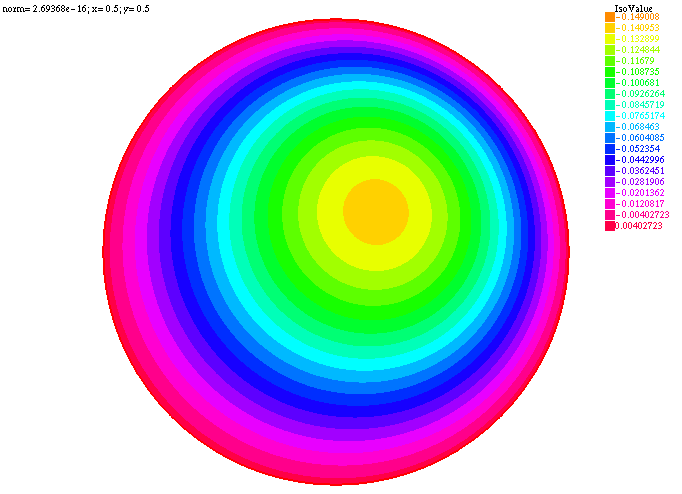
\includegraphics[scale=0.7]{0505.png}
	\caption{Converged solution of source position}
	\label{0505}
\end{figure}
We can see on figure \ref{0505} that the position has been found by the algorithm (top left corner) and the colors represent the values of the function $\phi$ where the maximum is on the source as expected.

Let's see how many iterations it takes for the  loop to converge with a convergence criteria of $10^{-16}$.\\
\begin{center}
$\begin{array}{|c|c|}
	\hline
	\text{Number of points} & \text{Iterations} \\
	\hline
	40 & 45\\
	80 & 46\\
	160 & 45 \\
	320 & 46\\
	\hline
\end{array}$
\end{center}

As we can see, the number of iterations needed to converge do not depends on the size of the mesh.

\subsection{Second test case}

For the second test case, we take $(0.95,0)$ as the coordinates of the source.\\
\begin{figure}[H]
	\centering
	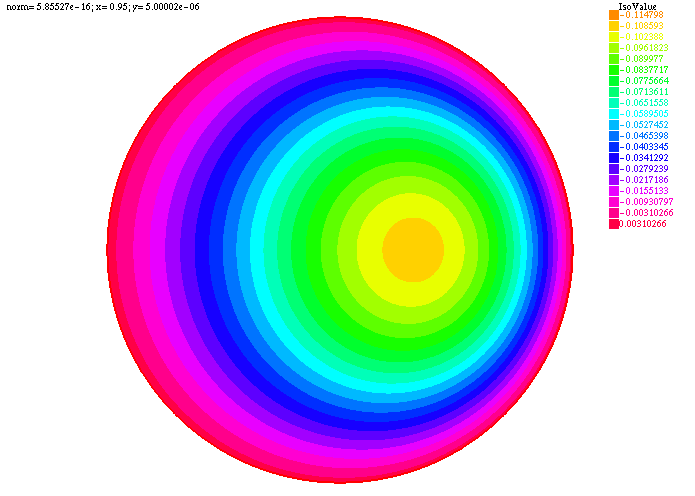
\includegraphics[scale=0.7]{0950.png}
	\caption{Converged solution of source position}
	\label{0950}
\end{figure}
On the top left corner we can see that the position of the source has been found. However the maximum of the function $\phi$ is not at this position. This is because we have a boundary condition that impose $\left.\Phi\right|_{\partial\Omega}=0$.

 

%% The Appendices part is started with the command \appendix;
%% appendix sections are then done as normal sections
\appendix

%\section{Section in Appendix}
%\label{appendix-sec1}

%% References with bibTeX database:

\bibliographystyle{elsarticle-num}
% \bibliographystyle{elsarticle-harv}
% \bibliographystyle{elsarticle-num-names}
% \bibliographystyle{model1a-num-names}
% \bibliographystyle{model1b-num-names}
% \bibliographystyle{model1c-num-names}
% \bibliographystyle{model1-num-names}
% \bibliographystyle{model2-names}
% \bibliographystyle{model3a-num-names}
% \bibliographystyle{model3-num-names}
% \bibliographystyle{model4-names}
% \bibliographystyle{model5-names}
% \bibliographystyle{model6-num-names}

\bibliography{bibliography}
\end{document}

%%
%% End of file `elsarticle-template-num.tex'.
